% lutorch_ex library report.
% Build: latexmk -pdf -interaction=nonstopmode -halt-on-error lutorch_ex_report_izhikevich_2026-10-09.tex
% fig_curves_v2.pdf is Figure 4, plotted from the val_bpb histories of the nine runs; the code is
% src/spiky/lutorch_ex/.
%
% The report goes from the smallest element to the full system (Figure 1):
%   1 one table, 2 lookup variants, 3 heads and the multi-head LUT, 4 the wrapper,
%   5 training (gradients and regularizers), 6 the int8 lookup and decode, 7 experiments.
% Vocabulary (software side): table, lookup variant (a ``cartridge'' in the code), head, multi-head LUT, wrapper, layer.
% Code identifiers (nap, tph, compress, decompress, cell_tv, read_top_n, export_deployment, ...) are unchanged.
\documentclass[11pt]{article}
\usepackage[margin=1in]{geometry}
\usepackage{lmodern}
\usepackage[T1]{fontenc}
\usepackage{amsmath,amssymb}
\usepackage{booktabs,array,tabularx}
\usepackage{xcolor}
\usepackage{listings}
\usepackage{graphicx}
\usepackage{caption}
\usepackage{tikz}
\usetikzlibrary{positioning,arrows.meta,backgrounds,fit,calc}
\usepackage[numbers]{natbib}
\usepackage{hyperref}
\hypersetup{colorlinks=true,linkcolor=black,citecolor=blue!60!black,urlcolor=blue!60!black,
  pdftitle={The lutorch\_ex library},pdfauthor={Anatoly Starostin}}
\captionsetup{font=small,labelfont=bf,skip=6pt}
\setlength{\parindent}{0pt}
\setlength{\parskip}{6pt}
\renewcommand{\arraystretch}{1.45}
\emergencystretch=2.5em
\renewcommand{\topfraction}{0.85}
\renewcommand{\textfraction}{0.1}
\renewcommand{\bottomfraction}{0.5}
\setcounter{topnumber}{3}
\setcounter{totalnumber}{4}
% typewriter with a line-break opportunity after every underscore and slash (long class and file names)
\DeclareRobustCommand{\code}[1]{{\renewcommand{\_}{\textunderscore\allowbreak}\texttt{#1}}}
\newcommand{\term}[1]{\textbf{#1}}
\newcolumntype{L}[1]{>{\raggedright\arraybackslash}p{#1}}
\newcommand{\sgn}{\operatorname{sgn}}
% \needlines{n}: start a new page here if fewer than n lines are left on the current one
\newcommand{\needlines}[1]{\par\ifdim\dimexpr\pagegoal-\pagetotal\relax<#1\baselineskip \newpage\fi}
\lstset{basicstyle=\ttfamily\footnotesize,columns=fullflexible,breaklines=true,frame=single,language=Python,
        keywordstyle=\color{blue!60!black},commentstyle=\color{green!40!black},showstringspaces=false,
        aboveskip=6pt,belowskip=4pt,xleftmargin=2pt}
\title{\vspace{-2.5em}\textbf{The \code{lutorch\_ex} library}\\[2pt]\large Multi-head lookup tables in PyTorch, from one table to the full model}
\author{Anatoly Starostin, DeepSpike Inc.\\[3pt]\normalsize October 2026}
\date{}
\begin{document}
\maketitle
\vspace{-3.5em}

\section*{Abstract}

\code{lutorch\_ex} is a small PyTorch library that replaces the feed-forward network (FFN) of a
transformer layer with lookup tables (LUTs). An FFN multiplies its input by two weight matrices. The
replacement performs a simpler operation. It turns the input into a small number of sign bits, uses those
bits as addresses into many small learnable tables, and adds up the rows that the addresses select. The
lookup itself needs no matrix multiplication. In a sweep of eight lookup variants trained for 48{,}000
steps, with one seed per configuration, the best lookup variant of the library reaches a slightly lower
validation loss than the dense FFN ($1.0865$ against $1.0894$ bits per byte). Its 8-bit version reaches
$1.0899$ bits per byte, the same as the dense FFN within the variation between runs.

\section*{How the report is organized}

The report builds the library from its smallest element to the full system, and each level contains the
one before it (Figure~\ref{fig:levels}). Sections~\ref{sec:table} to~\ref{sec:projection} go through the
levels: one table, the lookup variants (the rules for what a table returns), the heads and the multi-head LUT,
and the wrapper, which gives the multi-head LUT the interface of an FFN. Two further sections apply to
all of these levels and are not shown in the figure: Section~\ref{sec:training} describes training, and
Section~\ref{sec:quant} describes the same computation with 8-bit tables. Section~\ref{sec:ml} reports the
experiments with the full model. Table~\ref{tab:notation} collects the notation.

\begin{figure}[!htb]
\centering
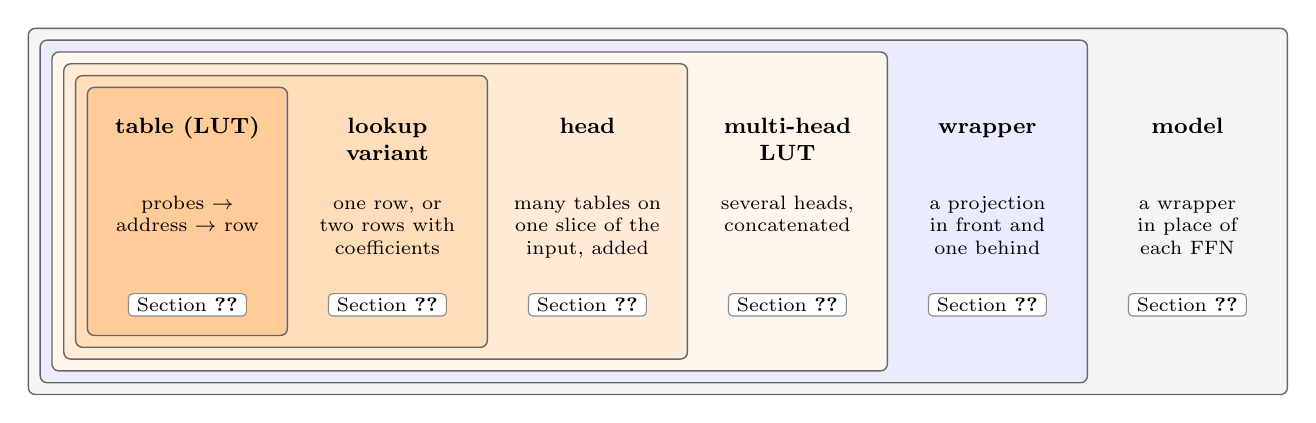
\begin{tikzpicture}[x=1mm, y=1mm,
  lvlname/.style={font=\footnotesize\bfseries, align=center, text width=21mm, anchor=north, inner sep=0pt},
  lvlhint/.style={font=\scriptsize, align=center, text width=21mm, anchor=north, inner sep=0pt},
  sectag/.style={draw=black!45, fill=white, rounded corners=1.5pt, font=\scriptsize, inner xsep=3pt, inner ysep=1.6pt}]
\def\W{25.4}% width of one label column, in mm
\def\D{1.5}%  inset between two nested boxes
\def\H{31.5}% height of the innermost box
% the nested boxes, drawn from the outermost to the innermost
\foreach \k/\fillcol in {6/black!4, 5/blue!8, 4/orange!7, 3/orange!16, 2/orange!27, 1/orange!40}{
  \draw[draw=black!60, line width=0.5pt, rounded corners=2.5pt, fill=\fillcol]
    ({-(\k-1)*\D},{-(\k-1)*\D}) rectangle ({\k*\W},{\H+(\k-1)*\D});
}
% one label column per box: name, a few words, section number
\foreach \k/\lname/\lhint/\lsec in {
  1/{table (LUT)}/{probes $\to$ address $\to$ row}/sec:table,
  2/{lookup\\variant}/{one row, or two rows with coefficients}/sec:variants,
  3/{head}/{many tables on one slice of the input, added}/sec:heads,
  4/{multi-head\\LUT}/{several heads, concatenated}/sec:heads,
  5/{wrapper}/{a projection in front and one behind}/sec:projection,
  6/{model}/{a wrapper in place of each FFN}/sec:ml}{
  \node[lvlname] at ({(\k-0.5)*\W},{\H-3.5}) {\strut\lname};
  \node[lvlhint] at ({(\k-0.5)*\W},{\H-13.5}) {\strut\lhint};
  \node[sectag, anchor=south] at ({(\k-0.5)*\W},2.4) {Section~\ref{\lsec}};
}
\end{tikzpicture}
\caption{The levels of the library, from the smallest element to the full system. Each box contains the
box to its left: a lookup variant is a table together with the rule for what it returns, a head is a group of
tables, a multi-head LUT is a group of heads, and so on. Sections~\ref{sec:table}
to~\ref{sec:projection} follow the boxes from left to right, and Section~\ref{sec:ml} reports
experiments with the full model.}
\label{fig:levels}
\end{figure}

% ======================================================================================================
\section{One table}
\label{sec:table}

This section describes the innermost box of Figure~\ref{fig:levels}: a single lookup table.

A lookup table does its work with memory instead of arithmetic. A matrix layer multiplies its input by
weights and adds up the products. A table instead computes an \term{address} from its input and returns
the vector that is stored at that address. This operation is called a \term{lookup}. The address must be
cheap to compute, and inputs that are similar to each other should usually receive the same address. A
hash function with this property is called a locality-sensitive hash (LSH)~\citep{lsh}. The hash function
used in this library consists of a small number of sign bits.

The construction comes from Izhikevich's \emph{Spiking Manifesto}~\citep{manifesto}. A spiking network
stores a very large number of synapses, but at any moment it uses only the synapses of the neurons that
have fired. A table lookup works in the same way: the table is large, and each input uses only one row of
it. In the Manifesto, the information is carried by the order in which the neurons fire. An address made
of sign bits encodes this order, because each bit records which of two neurons fired first.

\textbf{From the input to an address.} A table receives a vector $z\in\mathbb{R}^{d_\text{in}}$ as its
input (Figure~\ref{fig:table}). It examines $z$ with a small number of \term{probes}. The code calls the
number of probes \code{nap}. Each probe computes one number $u_j$ from $z$. There are two kinds of probe.
A probe on an \term{anchor pair} $(a_j,b_j)$ compares two coordinates of $z$, $u_j=z[a_j]-z[b_j]$. A
probe on a \term{single anchor} $a_j$ uses one coordinate, $u_j=z[a_j]$. An \term{anchor} is a position
in $z$, that is, the index of one coordinate. The anchors are chosen at random when the table is created,
and training does not change them.

Each probe produces one bit: the bit is 1 if $u_j>0$, and 0 otherwise. The \code{nap} bits, written next
to each other, form the address $c$. The address is an integer between $0$ and $K-1$, where
$K=2^{\text{nap}}$.

\textbf{From the address to a row.} The table has $K$ rows, one for each address. Row $c$ is a learnable
vector $W[c]\in\mathbb{R}^{d_\text{out}}$. In the simplest case, the lookup returns this row, so the
table maps the input $z$ to the row $W[c(z)]$. A table with \code{nap} probes therefore divides its
inputs into $K$ classes, and it stores one vector for each class.

\begin{figure}[t]
\centering
\resizebox{0.96\linewidth}{!}{%
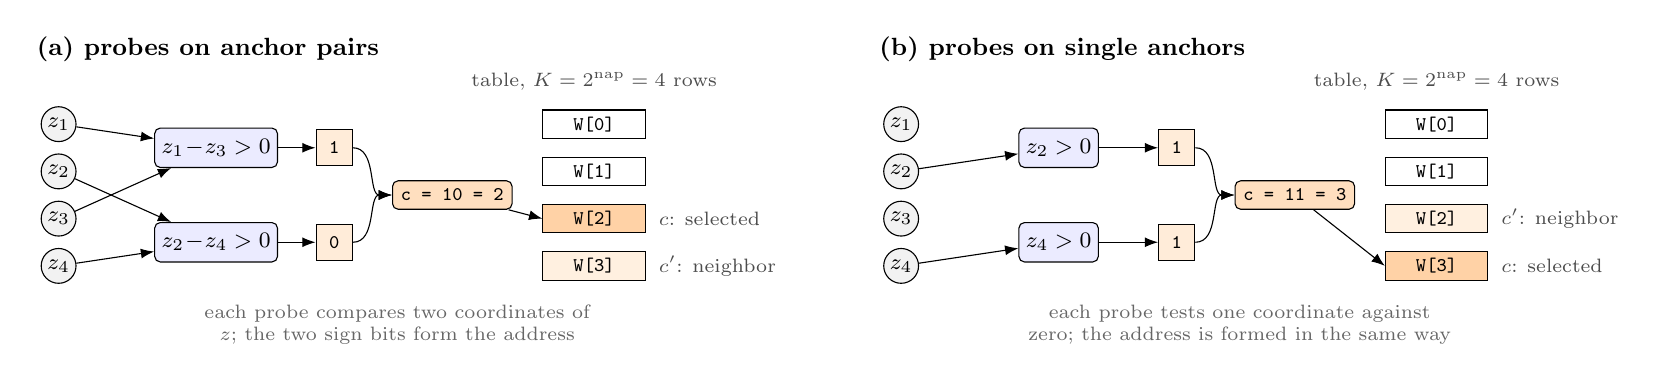
\begin{tikzpicture}[>=Latex, font=\footnotesize,
  coord/.style={draw, circle, inner sep=1.2pt, minimum size=4.4mm, fill=black!5},
  cmp/.style={draw, rounded corners=2pt, inner sep=2.5pt, minimum height=5mm, fill=blue!8},
  bit/.style={draw, inner sep=2pt, minimum size=4.6mm, fill=orange!15, font=\scriptsize\ttfamily},
  idx/.style={draw, rounded corners=2pt, fill=orange!25, inner sep=3pt, font=\scriptsize\ttfamily},
  row/.style={draw, minimum width=13mm, minimum height=3.6mm, inner sep=0pt, font=\scriptsize\ttfamily},
  tag/.style={font=\scriptsize, text=black!70},
  note/.style={font=\scriptsize, text=black!60, align=center, text width=58mm}]
% ================= panel (a): anchor pairs =================
\begin{scope}
\node[font=\small\bfseries, anchor=west] at (-0.4,2.75) {(a) probes on anchor pairs};
\foreach \i/\y in {1/1.8,2/1.2,3/0.6,4/0.0}{\node[coord] (z\i) at (0,\y) {$z_{\i}$};}
\node[cmp] (c1) at (2.0,1.5) {$z_1\!-\!z_3>0$};
\node[cmp] (c2) at (2.0,0.3) {$z_2\!-\!z_4>0$};
\draw[->] (z1) -- (c1); \draw[->] (z3) -- (c1);
\draw[->] (z2) -- (c2); \draw[->] (z4) -- (c2);
\node[bit] (b1) at (3.5,1.5) {1};
\node[bit] (b2) at (3.5,0.3) {0};
\draw[->] (c1) -- (b1); \draw[->] (c2) -- (b2);
\node[idx] (ix) at (5.0,0.9) {c = 10 = 2};
\draw[->] (b1.east) to[out=0,in=180] (ix.west);
\draw[->] (b2.east) to[out=0,in=180] (ix.west);
\foreach \r/\y in {0/1.8,1/1.2,2/0.6,3/0.0}{\node[row] (r\r) at (6.8,\y) {W[\r]};}
\node[row, fill=orange!35] (rc) at (6.8,0.6) {W[2]};
\node[row, fill=orange!12] (ra) at (6.8,0.0) {W[3]};
\node[tag, anchor=west] at (7.5,0.6) {$c$: selected};
\node[tag, anchor=west] at (7.5,0.0) {$c'$: neighbor};
\node[tag, anchor=south] at (6.8,2.1) {table, $K=2^{\text{nap}}=4$ rows};
\draw[->] (ix) -- (rc.west);
\node[note] at (4.3,-0.75) {each probe compares two coordinates of $z$; the two sign bits form the address};
\end{scope}
% ================= panel (b): single anchors =================
\begin{scope}[xshift=10.7cm]
\node[font=\small\bfseries, anchor=west] at (-0.4,2.75) {(b) probes on single anchors};
\foreach \i/\y in {1/1.8,2/1.2,3/0.6,4/0.0}{\node[coord] (s\i) at (0,\y) {$z_{\i}$};}
\node[cmp] (d1) at (2.0,1.5) {$z_2>0$};
\node[cmp] (d2) at (2.0,0.3) {$z_4>0$};
\draw[->] (s2) -- (d1);
\draw[->] (s4) -- (d2);
\node[bit] (e1) at (3.5,1.5) {1};
\node[bit] (e2) at (3.5,0.3) {1};
\draw[->] (d1) -- (e1); \draw[->] (d2) -- (e2);
\node[idx] (jx) at (5.0,0.9) {c = 11 = 3};
\draw[->] (e1.east) to[out=0,in=180] (jx.west);
\draw[->] (e2.east) to[out=0,in=180] (jx.west);
\foreach \r/\y in {0/1.8,1/1.2,2/0.6,3/0.0}{\node[row] (q\r) at (6.8,\y) {W[\r]};}
\node[row, fill=orange!35] (qc) at (6.8,0.0) {W[3]};
\node[row, fill=orange!12] (qa) at (6.8,0.6) {W[2]};
\node[tag, anchor=west] at (7.5,0.0) {$c$: selected};
\node[tag, anchor=west] at (7.5,0.6) {$c'$: neighbor};
\node[tag, anchor=south] at (6.8,2.1) {table, $K=2^{\text{nap}}=4$ rows};
\draw[->] (jx) -- (qc.west);
\node[note] at (4.3,-0.75) {each probe tests one coordinate against zero; the address is formed in the same way};
\end{scope}
\end{tikzpicture}}
\caption{One lookup table with two probes (\code{nap}$=2$), for each of the two kinds of probe. A probe
yields one sign bit. The bits, most significant first, form the address $c$, which selects one learnable
row of the table. The table has $K=2^{\text{nap}}=4$ rows. The probe with the smallest margin is the least
certain one. If its bit is inverted, the address selects the neighbor row $c'$ (shown in a lighter
color). A weighted retrieval (Section~\ref{sec:variants}) also fetches this row. (a) A probe on an anchor pair compares two coordinates of
$z$. (b) A probe on a single anchor tests one coordinate against zero.}
\label{fig:table}
\end{figure}

\textbf{Margins and the neighbor row.} The magnitudes $|u_j|$ are used as well. The magnitude $|u_j|$
is called the \term{margin} of bit $j$. It measures how far the input is from the point where bit $j$
changes its value. The smallest margin of a table, $u^\star=\min_j|u_j|$, is called the \term{deciding
margin}, and the bit with this margin is the least certain bit of the address. If this bit is inverted,
the result is a second address $c'$, which selects the \term{neighbor row}. The neighbor row is the row
that the input would select after the smallest change of the input that changes the address. A table
passes three things on to the next level: the address $c$, the margins $u_j$, and the neighbor address
$c'$. The lookup variants of Section~\ref{sec:variants} use no other information about the input.

\textbf{Two kinds of probe.} The kind of probe is chosen when a multi-head LUT
(Section~\ref{sec:heads}) is built, and all of its tables use the same kind. The default kind is the
anchor pair. It is the comparison used in the Manifesto (its Eq.~1), in which the bit records which of
two neurons fired first. The other kind is the single anchor, which tests the sign of one coordinate.
Section~\ref{sec:projection} compares the two kinds, because the result of the comparison depends on what
is placed in front of the tables.

% ======================================================================================================
\section{Lookup variants: what a table returns}
\label{sec:variants}

This section describes the next box of Figure~\ref{fig:levels}. Section~\ref{sec:table} ended with the
simplest lookup, in which the table returns the selected row $W[c]$. A table can return more than this
row. It can also fetch the neighbor row, and it can multiply each row by a coefficient. A \term{lookup
variant} is the rule that fixes these choices. (The code calls a lookup variant a \emph{cartridge}; this
report uses that word only for the Python classes.) The lookup variants are interchangeable: when one
lookup variant is replaced by another, nothing else in the system changes. Section~\ref{sec:oneformula}
gives the single formula that all lookup variants share. The rest of the report needs only that part.
Section~\ref{sec:generations} describes the lookup variants of the library one by one, and it can be
skipped at first.

\subsection{One formula, two ways to use it}
\label{sec:oneformula}

For one table, every lookup variant computes a vector $f$, which is the \term{contribution} of the table to
the output:
\begin{equation}\label{eq:retrieval}
  f=a\,W[c]+b\,W[c'] .
\end{equation}
Here $W[c]$ is the selected row, and $W[c']$ is the neighbor row, whose address differs from $c$ in the
least certain bit. The coefficients $a$ and $b$ are numbers. They depend on the input only through the
margins of the table. The formula is used in two ways.
\begin{description}\itemsep2pt
\item[Hard lookup.] The contribution is the selected row alone, that is, $a=1$ and $b=0$. The row is
  used as it is stored, without any multiplication. This is the cheapest possible lookup.
\item[Weighted retrieval.] Both rows are fetched, and each row is multiplied by its coefficient. The
  neighbor row receives a larger share of the sum when the deciding margin is smaller. The reason is
  that, with a small margin, a small change of the input would have selected the neighbor row instead.
\end{description}
A weighted retrieval uses Equation~\eqref{eq:retrieval} both in training and in decode (inference). A
hard lookup also uses the neighbor row and the coefficients, but only during training, where they are
needed to compute the gradient (Section~\ref{sec:gradient}).

\subsection{The lookup variants of the library}
\label{sec:generations}

The library has two families of lookup variants (Table~\ref{tab:matrix}). The Manifesto lookup variants
compute the coefficients from the deciding margin with an \term{uncertainty function} $U$. The argument
\code{uncertainty\_func} chooses $U$: a fixed function (\code{"rational"}, the default), or a function
with two learnable temperatures (\code{"softsign"}). The confidence lookup variants also use all the
other margins of the table. The Manifesto lookup variants are available both as a hard lookup and as a
weighted retrieval. The confidence lookup variants are available only as a weighted retrieval.

\begin{table}[htb]
\centering\small
\setlength{\tabcolsep}{7pt}
\begin{tabular}{@{}L{29mm}L{27mm}L{70mm}L{21mm}@{}}
\toprule
lookup variant & $a$, \ $b$ & defined by & learned scalars \\
\midrule
Manifesto, rational & $1-U$, \ $U$ & $U=0.5/(1+u^\star)$ & none \\
Manifesto, soft-sign & $1-U$, \ $U$ & $U=\sigma(-2\rho/T_\text{sel})$ \ with \ $\rho=u^\star/(T_\text{soft}+u^\star)$ & $T_\text{soft}$, $T_\text{sel}$ \\
Confidence, $n=1$ & $s$, \ $0$ & $s=\big(\sum_j m_j\big)\exp\!\big(\gamma\sum_j\log\sigma(\beta m_j)\big)$ & $\beta$, $\gamma$ \\
Confidence, $n=2$ & $s\,(1-v)$, \ $s\,v$ & the same $s$, \ and \ $v=\sigma(-2u^\star/\tau)$ & $\beta$, $\gamma$, $\tau$ \\
\bottomrule
\end{tabular}
\caption{The coefficients of the selected row ($a$) and of its neighbor ($b$) in
Equation~\eqref{eq:retrieval}, for the lookup variants of the library. Here $u^\star$ is the deciding margin,
$m_j=|u_j|$ are the margins of the table, $\sigma$ is the logistic function, and $n$ is the number of rows
retrieved per table. In a hard lookup these coefficients are used only in training.
Table~\ref{tab:classes} lists the classes.}
\label{tab:matrix}
\end{table}

\textbf{Manifesto, rational uncertainty.} The coefficient of the neighbor row is the fixed uncertainty function
$U$ of the Spiking Manifesto~\citep{manifesto}, applied to the deciding margin. $U$ equals $\tfrac12$
when the deciding margin is zero. In that case the two rows are equally plausible. $U$ decreases toward
zero as the margin grows. The hard lookup with this $U$, \code{ManifestoHardLUT}, is the rule of the
Manifesto as it was published. The weighted retrieval, \code{ManifestoSoftLUT}, goes beyond the
Manifesto. In the Manifesto, $U$ is used only to compute gradients during training, and inference uses
the plain sum of the selected rows (its Eq.~3 and Section III-A).

\textbf{Manifesto, soft-sign uncertainty.} This uncertainty function has the same role, but it is
learnable. Two parameters, the temperatures $T_\text{soft}$ and $T_\text{sel}$,
replace the fixed constants of $U$. The first temperature rescales the deciding margin into a number
$\rho$ between 0 and 1. The second temperature turns $\rho$ into the coefficient $U$, which is at most
$\tfrac12$. Both temperatures are learned. There is one pair of temperatures for each multi-head LUT
(Section~\ref{sec:heads}), and both start at the value $0.5$. They can also be kept fixed. The same two
classes, \code{ManifestoHardLUT} (hard lookup) and \code{ManifestoSoftLUT} (weighted retrieval), use
this $U$ when they are constructed with \code{uncertainty\_func="softsign"}.

\textbf{Confidence.} The Manifesto lookup variants use only the deciding margin. The confidence lookup
variants use all the margins of a table to estimate how much the table can be trusted for the present input. It
multiplies the contribution of the table by a \term{confidence score} $s$, which is the score of
LookupFFN~\citep{lookupffn}. The score is a product of two factors. The first factor is the sum of the
margins. It grows as the input moves away from the points where the bits change their values. The second
factor, the exponential, is equal to the product of $\sigma(\beta m_j)^\gamma$ over the probes of the
table. Each term of this product is close to $1$ when the margin is large, and it equals $2^{-\gamma}$
when the margin is zero. Every uncertain bit therefore reduces the contribution of the table. The scalar
$\beta$ determines which margins count as large, and the scalar $\gamma$ determines how strong the
reduction is.

The class \code{ConfidenceLUT} retrieves either one row or two rows per table ($n=1$ or $n=2$). With
$n=1$, the contribution of the table is the selected row multiplied by the score. With $n=2$, the
neighbor row is added as in the Manifesto weighted retrieval, and the score multiplies both rows. The coefficient $v$ of the
neighbor row is at most $\tfrac12$. It depends only on the deciding margin and on a temperature $\tau$.
The scalars $\beta$, $\gamma$ and $\tau$ are learned, and each multi-head LUT has one value of each. They
are stored as logarithms, and their initial values are $2$, $1$ and $0.5$.

% ======================================================================================================
\section{Heads and the multi-head LUT}
\label{sec:heads}

This section describes the next two boxes of Figure~\ref{fig:levels}. One table divides its inputs into
only $K$ classes, so a model uses many tables and adds up their contributions. The tables are grouped
into heads, and the heads are grouped into a multi-head LUT (the inner dashed box of
Figure~\ref{fig:projlut}).

\textbf{A head.} A \term{head} is a group of tables that all examine the same input vector. The code
calls the number of tables per head \code{tph}. Head $g$ receives its own slice $z_g$ of the input. The
slice has $d_\text{in}$ values, and all tables of the head apply their probes to it. Every table has its
own anchors, so every table forms its own address. Table $t$ of head $g$ forms the address $c_{g,t}$
from $z_g$, and it returns its contribution $f_{g,t}$ according to Equation~\eqref{eq:retrieval}. The
output of the head is the \emph{sum} of these contributions:
\begin{equation}\label{eq:head}
  y_g=\sum_{t=1}^{\text{tph}} f_{g,t}\ \in\mathbb{R}^{d_\text{out}}, \qquad g=1,\ldots,G .
\end{equation}
For a hard lookup, the output is the sum of the selected rows, $y_g=\sum_t W_{g,t}[c_{g,t}]$.

\textbf{A multi-head LUT.} A \term{multi-head LUT} consists of $G$ heads that work side by side. The
outputs of the heads are \emph{concatenated} into one vector:
\begin{equation}\label{eq:concat}
  y=[\,y_1,\ y_2,\ \ldots,\ y_G\,]\ \in\mathbb{R}^{G\,d_\text{out}} .
\end{equation}
As an alternative, the library can add the outputs of the heads into a single vector of width
$d_\text{out}$, $y=\sum_g y_g$. Together with the projections of Section~\ref{sec:projection}, the
multi-head LUT replaces an FFN.

\begin{figure}[t]
\centering
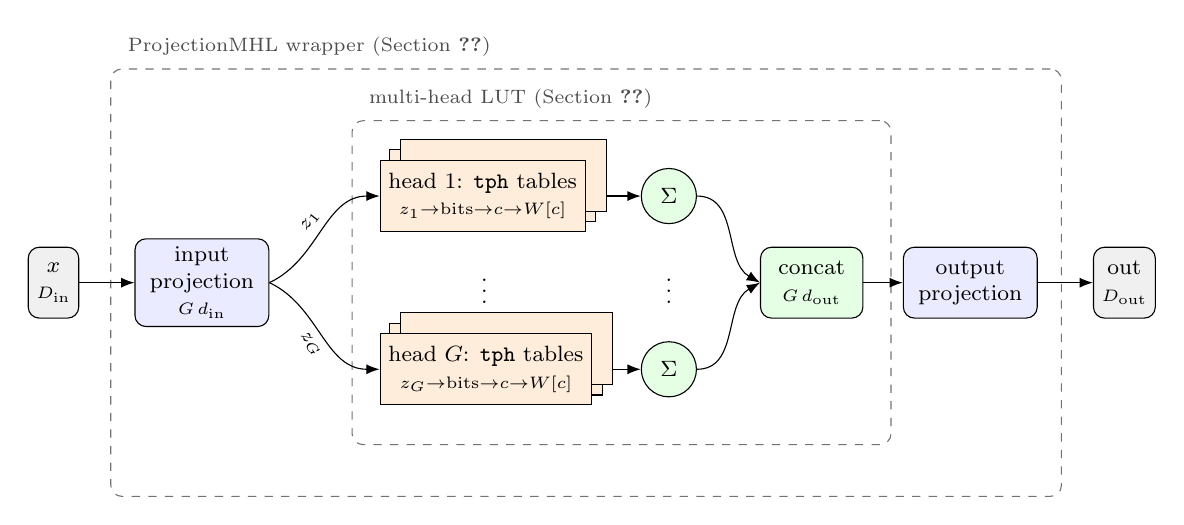
\begin{tikzpicture}[>=Latex, font=\footnotesize,
  box/.style={draw, rounded corners, align=center, inner sep=3pt, minimum height=9mm},
  io/.style={box, fill=black!6},
  proj/.style={box, fill=blue!8, minimum width=17mm},
  tbl/.style={draw, fill=orange!14, align=center, inner sep=3pt, minimum width=24mm, minimum height=9mm},
  sumop/.style={draw, circle, inner sep=1pt, minimum size=7mm, fill=green!10}]
\node[io] (x) {$x$\\$\scriptstyle D_\text{in}$};
\node[proj, right=7mm of x] (cmp) {input\\projection\\$\scriptstyle G\,d_\text{in}$};
\node[tbl, right=14mm of cmp, yshift=11mm] (t1) {head 1: \code{tph} tables\\$\scriptstyle z_1\to\text{bits}\to c\to W[c]$};
\node[tbl, right=14mm of cmp, yshift=-11mm] (t2) {head $G$: \code{tph} tables\\$\scriptstyle z_G\to\text{bits}\to c\to W[c]$};
\node at ($(t1)!0.5!(t2)$) {$\vdots$};
\node[sumop, right=7mm of t1] (s1) {$\Sigma$};
\node[sumop] (s2) at (s1 |- t2) {$\Sigma$};
\node at ($(s1)!0.5!(s2)$) {$\vdots$};
\node[box, fill=green!10, right=8mm of s1, yshift=-11mm, minimum width=13mm] (cat) {concat\\$\scriptstyle G\,d_\text{out}$};
\node[proj, right=5mm of cat] (dec) {output\\projection};
\node[io, right=7mm of dec] (y) {$\text{out}$\\$\scriptstyle D_\text{out}$};
\begin{scope}[on background layer]
  \foreach \t in {t1,t2}{ \foreach \dx in {1.3,2.6}{
    \draw[fill=orange!14, draw=black] ([xshift=\dx mm,yshift=\dx mm]\t.south east) rectangle ([xshift=\dx mm,yshift=\dx mm]\t.north west); }}
  \node[draw=black!55, dashed, rounded corners, fit=(t1)(t2)(s1)(s2)(cat), inner xsep=3.5mm, inner ysep=5mm] (mh) {};
  \node[draw=black!55, dashed, rounded corners, fit=(cmp)(mh)(dec), inner xsep=3mm, inner ysep=6.5mm] (wr) {};
\end{scope}
\node[font=\scriptsize, text=black!70, anchor=south west] at ([xshift=1mm,yshift=0.3mm]mh.north west) {multi-head LUT (Section~\ref{sec:heads})};
\node[font=\scriptsize, text=black!70, anchor=south west] at ([xshift=1mm,yshift=0.3mm]wr.north west) {ProjectionMHL wrapper (Section~\ref{sec:projection})};
\draw[->] (x) -- (cmp);
\draw[->] (cmp.east) to[out=25,in=180] node[above,sloped,font=\scriptsize]{$z_1$} (t1.west);
\draw[->] (cmp.east) to[out=-25,in=180] node[below,sloped,font=\scriptsize]{$z_G$} (t2.west);
\draw[->] ([xshift=2.6mm]t1.east) -- (s1);
\draw[->] ([xshift=2.6mm]t2.east) -- (s2);
\draw[->] (s1.east) to[out=0,in=150] (cat.west);
\draw[->] (s2.east) to[out=0,in=210] (cat.west);
\draw[->] (cat) -- (dec);
\draw[->] (dec) -- (y);
\end{tikzpicture}
\caption{A multi-head LUT (inner dashed box, Section~\ref{sec:heads}) inside the ProjectionMHL wrapper
(outer dashed box, Section~\ref{sec:projection}). The input projection
($D_\text{in}\to h_\text{in}d_\text{in}$) splits $x$ into the input slices $z_g$ of the heads. In each
head the probes turn $z_g$ into one address per table, and the contributions of the \code{tph} tables of
that head are added ($\Sigma$). The $G$ head outputs are concatenated, and the output projection
($h_\text{out}d_\text{out}\to D_\text{out}$) maps the concatenation to the output. (With
$h_\text{out}=1$, the head outputs are added into one slice instead.) The lookup variant determines how the
contribution of a table is computed. The wrapper does not use the internals of the multi-head LUT.}
\label{fig:projlut}
\end{figure}

\textbf{How large is a multi-head LUT?} A multi-head LUT has $G\times\code{tph}$ tables, and each table
has $2^{\text{nap}}$ rows. With 8 heads, 64 tables per head and \code{nap}$=8$, which are the sizes used
in Section~\ref{sec:ml}, the total is $8\times64\times256=131{,}072$ rows. Every row holds
$d_\text{out}$ values. With $d_\text{out}=48$, the tables therefore hold $6.3$ million values. In the
six-layer model of Section~\ref{sec:ml}, the tables of the six layers hold $37.7$ million values
together, which is more than half of the $68.2$ million parameters of the model. The tables are large,
but one input vector uses only a small part of them: one or two rows from each table.

\begin{table}[htb]
\centering\small
\renewcommand{\arraystretch}{1.3}
\setlength{\tabcolsep}{8pt}
\begin{tabular}{@{}L{26mm}L{100mm}L{24mm}@{}}
\toprule
name & meaning & value in Section~\ref{sec:ml} \\
\midrule
\multicolumn{3}{@{}l}{\emph{One table (Section~\ref{sec:table})}} \\
$z$ & input vector of a table; all tables of a head share it & \\
\code{nap} & number of probes per table, which is also the number of address bits & 8 \\
$K=2^{\text{nap}}$ & number of rows per table & 256 \\
$u_j$, $|u_j|$ & value of probe $j$, and the margin of its bit & \\
$u^\star$ & deciding margin: the smallest of the margins of a table & \\
$c$, $c'$ & address of the selected row, and of its neighbor row & 8 bits each \\
$W[c]$ & row $c$ of a table: $d_\text{out}$ learnable values & \\
\addlinespace[3pt]
\multicolumn{3}{@{}l}{\emph{One lookup variant (Section~\ref{sec:variants})}} \\
$a$, $b$ & coefficients of the selected row and of its neighbor row & \\
$f$ & contribution of one table, $a\,W[c]+b\,W[c']$ & \\
$n$ & number of rows retrieved per table by a confidence lookup variant (\code{read\_top\_n}) & 1 or 2 \\
\addlinespace[3pt]
\multicolumn{3}{@{}l}{\emph{Heads and the multi-head LUT (Section~\ref{sec:heads})}} \\
\code{tph} & number of tables per head & 64 \\
$G$ & number of heads in a multi-head LUT & 8 \\
$d_\text{in}$ & width of the input slice $z_g$ of a head & 48 \\
$d_\text{out}$ & width of a row, which is also the width of the output $y_g$ of a head & 48 \\
\addlinespace[3pt]
\multicolumn{3}{@{}l}{\emph{The wrapper (Section~\ref{sec:projection})}} \\
$D_\text{in}$, $D_\text{out}$ & input and output widths of the wrapper & 384 \\
$h_\text{in}$, $h_\text{out}$ & number of input slices and of output slices; both equal $G$ in the usual case & 8 \\
$B$ & number of input vectors in a batch & \\
\bottomrule
\end{tabular}
\caption{Notation, in the order of the levels of Figure~\ref{fig:levels}. Names in typewriter font are
the names used in the code.}
\label{tab:notation}
\end{table}

\textbf{How these heads compare with attention heads.} The name and the arrangement follow multi-head
attention. In a Transformer, the vector of width $d_\text{model}$ is projected into $h$ attention heads.
Each attention head works in its own narrow space of width $d_\text{model}/h$, the heads do not exchange
information, and their outputs are concatenated and projected back to the model width. A multi-head LUT
is arranged in the same way. It has $G$ heads, each head works on its own narrow slice, the heads do not
exchange information, and their outputs are concatenated as in Equation~\eqref{eq:concat}. The
projections in front of the heads and behind them are the subject of Section~\ref{sec:projection}. Even
the sizes are similar: the original Transformer has 8 attention heads of width 64 in a model of width
512, and the model of Section~\ref{sec:ml} has 8 heads of width 48 in a model of width 384.

The two kinds of head differ in what a head computes. An attention head combines information from different
tokens: for each token, it forms a weighted sum of value vectors that come from the other positions of
the sequence. A head of a multi-head LUT works on one token at a time, as an FFN does. Its output,
Equation~\eqref{eq:head}, is a sum of table rows selected by that token alone, and no other position is
involved. The heads of this report are therefore not attention heads. Where both kinds appear, the
report writes ``attention heads'' for the latter.

% ======================================================================================================
\section{The ProjectionMHL wrapper: input and output projections}
\label{sec:projection}

This section describes the wrapper, which is the last box of the library in Figure~\ref{fig:levels}. A
multi-head LUT works on $G$ narrow slices, but the model around it works on a single vector of the model
width. The class \code{ProjectionMHL}, the wrapper, connects the
two (Figure~\ref{fig:projlut}). It places one linear map in front of the multi-head LUT and another
linear map behind it. The first map is the \term{input projection}, and the second is the \term{output
projection}. (The code calls them \code{compress} and \code{decompress}.) Seen from the outside, the
wrapper takes a vector of width $D_\text{in}$ and returns a vector of width $D_\text{out}$, as an FFN
does. The two widths are separate arguments of the wrapper, and they may be different. The data path is
\[
  x\in[B,D_\text{in}]\xrightarrow{\ \substack{\text{input}\\\text{projection}}\ } z\in[B,h_\text{in},d_\text{in}]
  \xrightarrow{\ \substack{\text{multi-head}\\\text{LUT}}\ } y\in[B,h_\text{out},d_\text{out}]
  \xrightarrow{\ \substack{\text{output}\\\text{projection}}\ } \text{out}\in[B,D_\text{out}].
\]
Here the brackets give the shapes of the arrays, $B$ is the number of input vectors in a batch,
$h_\text{in}$ and $h_\text{out}$ are the numbers of input slices and output slices, and $d_\text{in}$ and
$d_\text{out}$ are the widths of these slices. In the usual case, every head has its own input slice and
its own output slice, so $h_\text{in}=h_\text{out}=G$.\footnote{The two numbers can be different only
when one of them is $1$. The library rejects every other combination. With $h_\text{in}=1$, the input
projection produces a single slice of width $d_\text{in}$, and all $G$ heads take this slice as their
input. With $h_\text{out}=1$, the outputs of the heads are added into a single slice of width
$d_\text{out}$, and the output projection receives this slice.} The two projections have different
purposes, which the next two subsections describe.

\subsection{The input projection}

\textbf{The input projection decides what the probes test.} A probe tests on which side of a hyperplane
the input lies. The set of hyperplanes that the probes can test depends on the kind of probe, and on
whether an input projection is present (Table~\ref{tab:planes}).

\begin{table}[htb]
\centering\small
\setlength{\tabcolsep}{8pt}
\begin{tabular}{L{34mm}L{52mm}L{58mm}}
\toprule
 & single anchors & anchor pairs \\
\midrule
no input projection & $x[a]>0$: a plane along a coordinate axis of the raw input & $x[a]-x[b]>0$: coefficients $\pm1$ and zero bias, the form of the Manifesto \\
with input projection & $w_a^\top x+b_a>0$: an arbitrary learned hyperplane & $(w_a-w_b)^\top x+(b_a-b_b)>0$: also arbitrary, with up to $\binom{d_\text{in}}{2}$ distinct planes per head \\
\bottomrule
\end{tabular}
\caption{The hyperplane that one probe tests. Here $w_a$ and $b_a$ are row $a$ of the input-projection
matrix and the corresponding bias, so that $z[a]=w_a^\top x+b_a$.}
\label{tab:planes}
\end{table}

Without an input projection, a probe on a single anchor can only test the sign of one coordinate of the
raw input. Such a test splits the input space along one coordinate axis. A probe on an anchor pair
compares two coordinates, so anchor pairs are much stronger in this case. With an input projection, every
coordinate of $z$ is itself a learned linear function of $x$. A probe on a single anchor then tests an
arbitrary learned hyperplane. This is the ``hyperplane LSH'' of the Manifesto, with learnable anchor
vectors (\citealp[Section VIII-H]{manifesto}). A probe on an anchor pair tests the difference of two such
functions, which is also an arbitrary hyperplane. With an input projection, the two kinds of probe
therefore test hyperplanes of the same type, and they differ only in the number of hyperplanes that are
available. The $d_\text{in}$ coordinates of a head give $d_\text{in}$ different hyperplanes to single
anchors, but up to $\binom{d_\text{in}}{2}$ different hyperplanes to anchor pairs. When more hyperplanes
are available, different tables are less likely to use the same few bits. Single anchors are therefore
somewhat weaker than anchor pairs even with an input projection, but the difference is not large.

\textbf{With a learned input projection, are anchor pairs still needed?} In principle, they are not
needed. A pair comparison $x[a]-x[b]>0$ is a hyperplane test in which the coefficient is $+1$ at position
$a$, $-1$ at position $b$, and zero at all other positions. A single anchor behind an input projection
could test the same hyperplane if the corresponding row of the projection matrix had this form. In
practice, the rows of the matrix do not take this form, because ordinary training has no reason to turn
a dense row into a row with one $+1$, one $-1$, and zeros. To obtain the pair form from a learned
projection, the library would need additional methods that it does not have. Examples are a strict
regularizer, or a straight-through estimator that maps the matrix entries to $\pm1$. (A straight-through
estimator is a training method that rounds a value in the forward pass, and computes the gradient in the
backward pass as if the value had not been rounded.)

For this reason, the library keeps both kinds of probe. The anchor pair is the mechanism of the Manifesto
in its original form: it compares the order of two coordinates. The anchor pair is also a special case
that is cheap to compute, and the whole design is built to take advantage of it. One address bit costs
two memory reads (one coordinate each) and one subtraction. The anchors are stored as integer positions,
and the bit has no trainable parameters of its own. The kernels of the library (the low-level routines
that carry out the computation) work in this way. A general hyperplane for every bit would instead cost a
dot product of length $d_\text{in}$, and it would need $d_\text{in}$ parameters. In the example of
Section~\ref{sec:heads}, with $d_\text{in}=48$, anchor pairs need about 4{,}000 subtractions per token and
layer, whereas general hyperplanes would need about 200{,}000 multiply-adds. The single anchor was added
to the library later, for flexibility. It is even cheaper than the anchor pair, but it is also somewhat
weaker.

\subsection{The output projection}

\textbf{The output projection keeps the rows narrow.} Section~\ref{sec:heads} showed that the number of
rows is determined by the numbers of heads, tables and probes. The size of the tables then depends on the
row width $d_\text{out}$. If the rows had the full width of the model, $d_\text{out}=384$, the tables of
that example would hold $50$ million values per layer. With $d_\text{out}=48$ they hold $6.3$ million
values. The rows are therefore kept narrow, and the output projection afterwards maps the concatenated
outputs of the heads to the model width. The cost of the output projection is one small dense matrix per
layer, with $0.15$ million parameters.

\textbf{Switching a projection off.} When the widths already match, one of the two projections can be
replaced by the identity map. The library does not allow both projections to be replaced at the same
time. By default, both projections are present. The output projection is initialized to zero, and the
input projection is initialized with random values from $\mathcal{N}(0,0.02)$.

\subsection{In code}

The classes of the library correspond to the levels of Figure~\ref{fig:levels}
(Table~\ref{tab:classes}). Each lookup variant is a class. An object of this class is a complete multi-head LUT
that uses one rule for the contribution of a table. All lookup variants have the same interface, which is
defined by the shapes of the arrays: a lookup variant maps an array of shape $[B,h_\text{in},d_\text{in}]$ to an
array of shape $[B,h_\text{out},d_\text{out}]$. The class \code{MultiHeadLUT} defines this interface. The
wrapper relies only on these shapes, and it does not use the internals of a lookup variant.

All lookup variants are also derived from one base class, \code{ManifestoLUT}. The base class holds the tables,
in an array $W$ of shape $G\times\code{tph}\times K\times d_\text{out}$, and the anchors. It also
provides the things that every lookup variant needs: the selected row, the margins, the neighbor row, and the
routing of the result of each head to its position in the output. The class of a lookup variant then defines two things
of its own. The first is the choice of the coefficients in Equation~\eqref{eq:retrieval}. The second is
the function that training differentiates (Section~\ref{sec:gradient}). Each of these classes, the
\term{reference} classes, is written in plain PyTorch and runs on the CPU and on CUDA. Each also exists
in a version whose name begins with \code{Fused}. A fused class computes the same mathematics in
hand-written CUDA kernels. It needs a CUDA input, and it never falls back to PyTorch: an input that its
kernels do not cover raises an error.

\begin{table}[htb]
\centering\small
\setlength{\tabcolsep}{8pt}
\begin{tabular}{@{}L{36mm}L{50mm}L{62mm}@{}}
\toprule
level & class & role \\
\midrule
lookup variant, Manifesto & \code{ManifestoHardLUT}, \code{ManifestoSoftLUT} & hard lookup, weighted retrieval; \code{uncertainty\_func="rational"} (the default) or \code{"softsign"} \\
lookup variant, confidence & \code{ConfidenceLUT}, \code{QuantisedConfidenceLUT} & weighted retrieval with $n=1$ or $n=2$ rows (\code{read\_top\_n}); the second trained for int8 tables (Section~\ref{sec:quant}) \\
lookup variant, fused & the prefix \code{Fused} before any of these four class names, for example \code{FusedManifestoHardLUT} & the same mathematics in hand-written CUDA kernels; CUDA input only \\
lookup variant, int8 decode & \code{Deployed\allowbreak QuantisedConfidenceLUT} & inference only, built from an export of \code{QuantisedConfidenceLUT} (Section~\ref{sec:quant}) \\
multi-head LUT & \code{MultiHeadLUT} & the interface of every lookup variant: $[B,h_\text{in},d_\text{in}]\to[B,h_\text{out},d_\text{out}]$ \\
 & \code{ManifestoLUT} & the base class of every lookup variant: tables, anchors, addresses, margins, routing of the head outputs \\
 & \code{LUTSpec} & the sizes of a multi-head LUT: the numbers of heads, tables per head and probes per table, and the widths \\
wrapper & \code{ProjectionMHL} & input projection, multi-head LUT, output projection \\
\bottomrule
\end{tabular}
\caption{The classes of the library, by level.}
\label{tab:classes}
\end{table}

The wrapper accepts any lookup variant, and the example below uses \code{ConfidenceLUT}. The wrapper maps an
array of shape $[N,D_\text{in}]$ to an array of shape $[N,D_\text{out}]$, so a batch of sequences must
first be flattened into a list of vectors:

\noindent\begin{minipage}{\linewidth}
\begin{lstlisting}
import torch
from spiky.lutorch_ex import LUTSpec, ConfidenceLUT, ProjectionMHL

spec = LUTSpec(h_in=8, h_out=8, tph=64, nap=8, d_in=48, d_out=48)  # 8 heads of 64 tables
mhl  = ConfidenceLUT(spec, seed=1, read_top_n=2)                    # the cartridge; 2 rows per table
ffn  = ProjectionMHL(mhl, d_model=384)           # or input_dim=..., output_dim=... (may differ)
x = torch.randn(4, 128, 384)                     # (B, T, D) activations
y = ffn(x.reshape(-1, 384)).reshape(x.shape)     # torch.Size([4, 128, 384])
\end{lstlisting}
\end{minipage}

Any other lookup variant class can be used in place of \code{ConfidenceLUT}; a fused class needs the
input on a CUDA device.

% ======================================================================================================
\section{Training: gradients and regularizers}
\label{sec:training}

Sections~\ref{sec:table} to~\ref{sec:projection} describe the forward computation, that is, how the
output is computed from the input. This section describes what training needs in addition: a way to
compute the gradient through a lookup, and two regularizers. Both topics concern the inner boxes of
Figure~\ref{fig:levels}, that is, the tables and their lookup variants.

\subsection{How the gradient reaches the input}
\label{sec:gradient}

Training needs the derivative of the contribution of a table, Equation~\eqref{eq:retrieval}, with respect
to the input $z$ of the table. The addresses $c$ and $c'$ are integers, and an integer-valued quantity
has no useful derivative. The coefficients $a$ and $b$, however, are smooth functions of $z$, because
they depend on $z$ through the margins. The gradient can therefore pass through the coefficients.

\textbf{Weighted retrieval.} In a weighted retrieval, the gradient with respect to the input passes
through $a$ and $b$ only. The selected row and the neighbor row both contribute to the output, so both
rows are updated by training.

\textbf{Hard lookup.} In a hard lookup, the coefficients are constants ($a=1$, $b=0$), so the output has
no useful derivative with respect to the input. A hard lookup therefore uses a different function in the
backward pass. In the backward pass, and only there, it uses Equation~\eqref{eq:retrieval} with the
coefficients of the weighted retrieval with the same uncertainty function. A function that is used in this way is
called a \term{surrogate}: it is a smooth function that replaces a function without a useful derivative.
The surrogate provides the gradient with respect to the input. The update of the table itself goes to
the selected row $c$ only.

\textbf{Manifesto.} With the coefficients $a=1-U$ and $b=U$ of Table~\ref{tab:matrix},
differentiating Equation~\eqref{eq:retrieval} gives
\[
  \frac{\partial\tilde f}{\partial z[a_{j^\star}]}=-\frac{\partial\tilde f}{\partial z[b_{j^\star}]}
  =U'(u^\star)\,\sgn(u_{j^\star})\,\big(W[c']-W[c]\big).
\]
Here $j^\star$ is the deciding probe, $a_{j^\star}$ and $b_{j^\star}$ are its two anchors, and the tilde
indicates the surrogate. The gradient with respect to the input is therefore nonzero only at the two
anchors of the deciding probe, and it has opposite signs at the two anchors (Eqs.~4 and~5 of the
Manifesto). This holds for both uncertainty functions, because both depend on the input only through the
deciding margin. With \code{"softsign"}, the two temperatures receive a gradient as well.

\textbf{Confidence.} In a confidence lookup variant, the gradient reaches the input only through the score $s$, which
depends on all \code{nap} margins, and for $n=2$ also through $v$, which depends on the deciding margin.
In this way, a table learns how much confidence to assign to its output. The gradient never tells the
table that a different row would have been a better choice.

\subsection{Regularizers}
\label{sec:reg}

Two regularizers are implemented in the base class \code{ManifestoLUT}, so every lookup variant with a
trainable table can use them (all except \code{DeployedQuantisedConfidenceLUT}, which is inference only).
Both are switched off by default. The first regularizer acts on the rows of a table, and the second acts
on whole tables.

\textbf{Row total variation.} The $K=2^{\text{nap}}$ rows of a table can be pictured as the corners of a
cube with \code{nap} dimensions, with one dimension for each address bit. Two rows are neighbors when
their addresses differ in a single bit, as the addresses $c$ and $c'$ do. When the input changes so that
one bit changes its value, the input moves from one row to a neighbor of that row. This is the smallest
change of the input that changes the address. It is therefore reasonable to require that such a change
alters the output only slightly. The regularizer expresses this requirement as a penalty on the mean
squared difference between neighboring rows:
\[
  \mathcal R_\text{TV}=\frac{1}{T\cdot\text{nap}\cdot2^{\text{nap}-1}}
  \sum_{t=1}^{T}\ \sum_{(c,c')}\big\|W_t[c]-W_t[c']\big\|_2^2 .
\]
Here $T=G\cdot\code{tph}$ is the number of tables. The inner sum runs over all pairs of rows whose
addresses differ in a single bit, and each pair is counted once. A table has
$\text{nap}\cdot2^{\text{nap}-1}$ such pairs, which explains the normalization factor. The method
\code{ManifestoLUT.cell\_tv} computes this penalty for one multi-head LUT. The function
\code{cell\_tv\_penalty(model)} averages the penalty over the multi-head LUTs of the model, and the
training loss adds $\lambda$ times this average. The penalty acts only on the values in the tables, and
it does not change the forward pass.

\textbf{Table dropout.} When the dropout rate $p$ is greater than zero (the argument
\code{table\_dropout\_rate}), training removes whole tables at random. For every sample, every head and
every table, an independent random decision keeps the table with probability $1-p$. The outputs of the
tables that are kept are multiplied by $1/(1-p)$, so the expected output does not change. A table that is
removed contributes nothing to the output or to the gradient for that sample. In a confidence lookup
variant, the dropout mask multiplies the score $s$, which has the same effect. In decode, and whenever gradients are
switched off, no table is removed and no output is rescaled.

% ======================================================================================================
\section{The int8 lookup and decode}
\label{sec:quant}

Sections~\ref{sec:table} to~\ref{sec:projection} describe the computation in floating point. This section
shows how the same computation is carried out with 8-bit tables and integer arithmetic, and how a trained
model is stored for decode. The change affects every level of Figure~\ref{fig:levels} from the table to
the wrapper: the rows of a table, the coefficients of the lookup variant, the sum of a head, and the output
projection.

\textbf{Why quantize?} Most of the parameters of a LUT model are in its tables. In the example of
Section~\ref{sec:heads}, the tables hold $6.3$ million values per layer. In the whole model, they hold
$37.7$ million of the $68.2$ million parameters. When the tables are stored as 8-bit integers (int8)
instead of 32-bit floating-point numbers (fp32), they need only a quarter of the memory.
\code{QuantisedConfidenceLUT} is the confidence lookup variant, with $n=1$ or $n=2$, that is trained so
that it can be decoded in this form; \code{FusedQuantisedConfidenceLUT} computes the same in CUDA
kernels. Its quantization mode is named \code{p2\_int8}, which stands for powers of two and
int8. The mode is selected by the argument \mbox{\code{quant\_mode="p2\_int8"}}.

\textbf{What \code{p2\_int8} does.} The mode converts the weighted retrieval
$s(1-v)\,W[c]+s\,v\,W[c']$ into integer arithmetic. It does this in three steps, one for each of the
three inner levels of Figure~\ref{fig:levels}.
\begin{enumerate}\itemsep2pt
\item \textbf{The rows of a table become int8.} Each row is stored as
  \[
    \hat W=\operatorname{clamp}\big(\operatorname{round}(W/2^{e}),\,-128,\,127\big),
    \qquad e=\lceil\log_2\max|W|\rceil-7 .
  \]
  The integer $e$ is called the \term{shared exponent}. There is one shared exponent for each head and
  each output component, and the maximum is taken over all tables and all rows of the head. This choice
  of $e$ makes the largest entry as large as an 8-bit integer allows.
\item \textbf{The coefficients of the lookup variant become powers of two.} The retrieval can be written as
  $s(1-v)\,(W[c]+r\,W[c'])$ with the ratio $r=v/(1-v)=e^{-2u^\star/\tau}$. The ratio is rounded to a
  power of two, $2^{-q}$, with $q=\operatorname{round}\big(2u^\star/(\tau\ln2)\big)$. The common factor
  $s(1-v)=s/(1+r)$ is rounded to $2^{k'}$, with $k'=\operatorname{round}(\log_2 s-c_q)$ and
  $c_q=\log_2(1+2^{-q})$. A table then adds $2^{k'}\hat W[c]+2^{k'-q}\hat W[c']$. This operation needs
  two shifts and one addition, and it needs no multiplication. With $n=1$ there is no neighbor row: the
  score itself is rounded, $k'=\operatorname{round}(\log_2 s)$, and a table adds $2^{k'}\hat W[c]$.
\item \textbf{The sum of a head becomes an integer sum.} The shifts are counted in units of $2^{-6}$, so
  that every shift is a shift to the left. The sum over the tables is kept in a 32-bit integer
  accumulator. Only one floating-point operation remains: the shared exponent is applied once, after the
  sum over the tables, as the factor $2^{e-6}$ for each output component.
\end{enumerate}

The scheme has a few limits. The exponents $q$ and $k'$ are computed from the margins in floating point.
Only the table lookup and the sum use integer arithmetic. The exponent $q$ is limited to at most $64$,
and $c_q$ is set to $0$ when $q\ge8$. The exponent $k'$ is kept between $-3$ and $4$. If $k'$ is below
this range, the table is skipped for that input, but it still receives its gradient. If $k'$ is above
this range, it is set to $4$. The neighbor row is omitted when $q>3$, that is, when its coefficient is
less than $\tfrac18$ of the coefficient of the selected row.

\textbf{Training is quantization-aware.} The model is trained with the rounding already applied: the
forward pass in training uses the rounded tables and the rounded coefficients. Rounding has no useful
derivative, so both roundings use a straight-through estimator. Like the surrogate of
Section~\ref{sec:gradient}, a straight-through estimator uses one function in the forward pass and
another function in the backward pass. The forward pass computes with the rounded values, and the
backward pass computes the gradient as if the values had not been rounded. The gradient therefore goes to
the floating-point \term{master tables}, from which the int8 tables are derived, and to the exact
coefficients $s(1-v)$ and $s\,v$. For this reason, the scalars $\beta$, $\gamma$ and $\tau$ continue to
be trained.

\textbf{Decode.} Because the rounding is already applied during training, decode computes the same
numbers as training, except for round-off errors. Preparing a trained model for decode therefore changes
only the way in which the model is stored. The function \code{export\_deployment} writes the int8 tables
to a file and discards the floating-point master tables. It also multiplies a copy of the
output-projection matrix by the factor $2^{e-6}$, so that the shared exponent becomes part of that
matrix. This multiplication is exact, because multiplying a floating-point number by a power of two
changes only its exponent. As a result, no separate step has to apply the shared exponent at run time.
The file contains the int8 tables, the anchors, the scalars $\beta$ and $\gamma$ (and $\tau$ when $n=2$)
and the two projections; the rest of the model is stored as it is. In the example, the tables of one
layer shrink from $24$~MiB to $6$~MiB (a MiB is $2^{20}$ bytes). The function \code{load\_deployment}
first calls a function supplied by the user, \code{make\_skeleton}, which builds the model on PyTorch's
\code{meta} device, a placeholder device on which arrays have shapes but occupy no memory. It then fills
the model from the file, so the floating-point tables are never allocated in memory. Each quantized
multi-head LUT becomes a \code{DeployedQuantisedConfidenceLUT}. In decode, it returns the integer
accumulator, and the output projection applies the shared exponent that was included in it. On a CUDA
input, the integer lookup is one hand-written kernel; on a CPU input, it is the PyTorch definition of the
same integer arithmetic.
\begin{lstlisting}
export_deployment(model, "m.lxq")
dep = load_deployment("m.lxq", make_skeleton, device="cuda").eval()
\end{lstlisting}

% ======================================================================================================
\section{Experiments: eight lookup variants and the dense FFN}
\label{sec:ml}

This section describes the outermost box of Figure~\ref{fig:levels}, the full model. It answers two
questions. How well do the lookup variants learn, compared with each other and with the dense FFN that
they replace? And how fast do they run?

\subsection{Setup}

The test model is a six-layer GPT. In every layer, the FFN is replaced by a \code{ProjectionMHL} wrapper
that contains the lookup variant under test. Eight configurations were trained, and they differ only in
the lookup variant. Each of them uses the fused class of its lookup variant. A ninth run, the baseline,
keeps the dense FFN. Table~\ref{tab:setup} lists the settings. The configuration files, the training
scripts, and a summary of every run (including the training time and the peak memory) are available on the
branch at
\url{https://github.com/anatoli-starostin/spiky/tree/research/lutorch_ex_fused_ablations/experiments/lutorch_ex_fused}.

\begin{table}[htb]
\centering\small
\renewcommand{\arraystretch}{1.3}
\setlength{\tabcolsep}{8pt}
\begin{tabular}{L{30mm}L{118mm}}
\toprule
item & value \\
\midrule
model & six-layer GPT (pre-norm blocks, rotary position embeddings, untied output layer), $d_\text{model}=384$, 6 attention heads; $68.2$M parameters with the multi-head LUTs, $35.8$M with the dense FFN \\
dense FFN & $384\!\to\!1536\!\to\!384$ with GELU, no bias, no dropout \\
wrapper & square: $D_\text{in}=D_\text{out}=d_\text{model}=384$ \\
multi-head LUT & $h_\text{in}=h_\text{out}=8$ heads, \code{tph}$=64$, \code{nap}$=8$, $d_\text{in}=d_\text{out}=48$, anchor pairs \\
initialization & seed 1; tables uniform in $[-10^{-3},10^{-3}]$ per head, input projection $\mathcal{N}(0,0.02)$, output projection zero \\
regularizers & multi-head LUTs only: row total variation with $\lambda=10$, and table dropout with $p=0.2$ (Section~\ref{sec:reg}) \\
optimizer & AdamW, learning rate $3\times10^{-4}$, $\beta=(0.9,0.95)$, weight decay $0.1$ (none on the tables and on the parameters with fewer than two dimensions), gradient clipping at $1.0$ \\
schedule & 48{,}000 steps; cosine schedule, $10\%$ warm-up, floor at $0.1\times$ the peak rate \\
batch & sequences of 512 tokens; 24{,}576 tokens per step (LUT runs: device batch 12, gradient accumulation 4; dense run: device batch 48), $1.18$ billion tokens in all \\
precision & fp32 throughout \\
validation & every 500 steps, on a fixed held-out set of 4{,}788 sequences \\
data & the \emph{NanoChat} setup: the ClimbMix text corpus as prepared by nanochat's data script, 170 shards; the runs read less than one pass of it \\
tokenizer & nanochat's RustBPE tokenizer, with a vocabulary of 32{,}768 entries trained by nanochat on the same corpus; the text is streamed and tokenized on the fly into sequences of 512 tokens, aligned to the beginning-of-sequence (BOS) token \\
\bottomrule
\end{tabular}
\caption{The settings of the nine runs.}
\label{tab:setup}
\end{table}

The metric is \code{val\_bpb}, the validation loss in bits per byte (bpb). It is the cross-entropy on a
fixed held-out set, measured in bits and divided by the number of \emph{bytes} of the text that the
tokens represent. (This is the bits-per-byte measure of nanochat.) Because the loss is divided by the
number of bytes and not by the number of tokens, the metric can be compared between models with different
tokenizers. A lower value is better.

\subsection{Results}

\begin{table}[!htb]
\centering\small
\setlength{\tabcolsep}{5pt}
\begin{tabular}{@{}L{60mm}L{40mm}rrr@{}}
\toprule
FFN replacement & lookup & params & \code{val\_bpb} & $\Delta$ vs.\ dense \\
\midrule
dense FFN, $384\!\to\!1536\!\to\!384$, GELU & none & 35.8M & 1.08936 & \\
\midrule
\code{FusedConfidenceLUT} $n=2$           & scored weighted retrieval & 68.2M & \textbf{1.08653} & $-0.0028$ \\
\code{FusedQuantisedConfidenceLUT} $n=2$  & the same, in int8 & 68.2M & 1.08986 & $+0.0005$ \\
\code{FusedConfidenceLUT} $n=1$           & scored single row & 68.2M & 1.09698 & $+0.0076$ \\
\code{FusedQuantisedConfidenceLUT} $n=1$  & the same, in int8 & 68.2M & 1.09928 & $+0.0099$ \\
\code{FusedManifestoSoftLUT}, soft-sign   & weighted retrieval with $U$ & 68.2M & 1.10954 & $+0.0202$ \\
\code{FusedManifestoSoftLUT}, rational    & weighted retrieval with $U$ & 68.2M & 1.11863 & $+0.0293$ \\
\code{FusedManifestoHardLUT}, rational    & hard lookup & 68.2M & 1.13242 & $+0.0431$ \\
\code{FusedManifestoHardLUT}, soft-sign   & hard lookup & 68.2M & 1.13780 & $+0.0484$ \\
\bottomrule
\end{tabular}
\caption{The nine runs at 48{,}000 steps, one seed each. Every run improves until its last evaluation, so
\code{val\_bpb} is both the final and the best value. ``Soft-sign'' and ``rational'' are the values of
\code{uncertainty\_func}. The baseline has the same backbone (6 layers, $d_\text{model}=384$, 6 attention
heads), data, tokenizer, schedule, batches of 24{,}576 tokens and seed, with a dense
$384\!\to\!1536\!\to\!384$ GELU network as the FFN and no regularizer (run \code{00\_vanilla}). The int8
lookup variants are trained with int8 rows and power-of-two coefficients (Section~\ref{sec:quant}). Each
fused class has the mathematics of its reference class.}
\label{tab:results}
\end{table}

\begin{figure}[!htb]
\centering
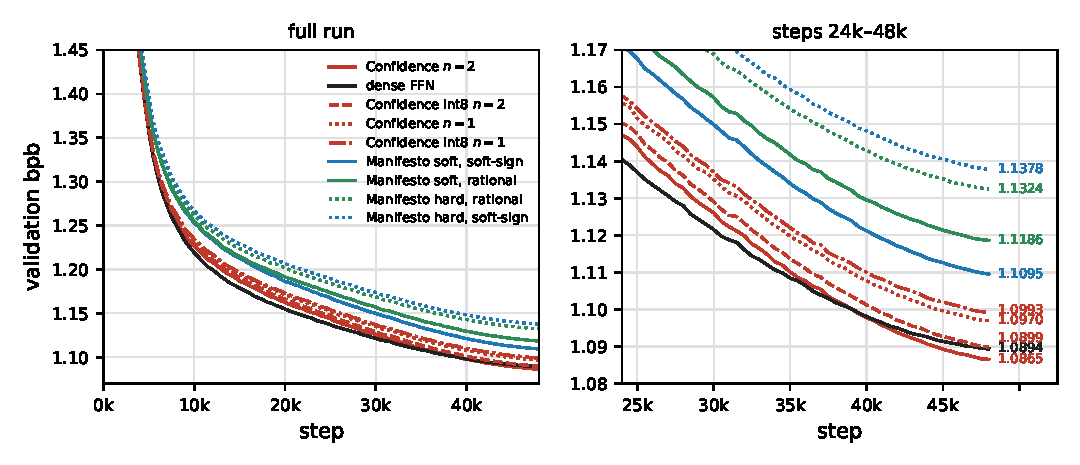
\includegraphics[width=\linewidth]{fig_curves_v2.pdf}
\caption{Validation loss in bits per byte for the nine runs. Left: the full run. Right: the second half,
with the final value of each run. Color marks the family (red confidence, blue Manifesto with the
soft-sign uncertainty function, green Manifesto with the rational one, black the dense FFN). Solid lines
retrieve two rows per table, and dotted lines one row (the two hard lookups, and confidence with $n=1$).
The dashed and the dash-dotted lines are the int8 lookup variants with $n=2$ and $n=1$.}
\label{fig:curves}
\end{figure}

Table~\ref{tab:results} and Figure~\ref{fig:curves} show five results. Each configuration was run once.
\code{FusedConfidenceLUT} with $n=1$ was also run with seeds 2 and 3, which gave $1.09682$ and $1.09460$
bpb. The standard deviation of the three runs, $0.0013$ bpb, shows how much a result can vary from one run
to the next.
\begin{enumerate}\itemsep0pt
\item \textbf{A weighted retrieval is better than a hard lookup.} With both uncertainty functions, the
  weighted retrieval has the lower loss: by $0.014$ bpb with the rational one, and by $0.028$ bpb with the
  soft-sign one. The learnable soft-sign function helps the weighted retrieval (by $0.009$ bpb), but not
  the hard lookup, which it makes worse by $0.005$ bpb.
\item \textbf{Two rows are better than one.} Among the confidence lookup variants, the form that also
  retrieves the neighbor row ($n=2$) is better than the form with a single scored row ($n=1$), by $0.010$
  bpb. Both forms multiply their rows by the score. This result therefore compares one row with two rows,
  and it does not compare a hard lookup with a weighted retrieval. The same result holds after
  quantization, by $0.009$ bpb. Both differences are seven to eight times the variation from run to run.
\item \textbf{The confidence score improves the result.} The Manifesto lookup variants weight the two rows
  according to the uncertainty of one bit only. The confidence lookup variants add the confidence score,
  and they do better: \code{FusedConfidenceLUT} with $n=2$ is ahead of the best Manifesto run (the weighted
  retrieval with the soft-sign function) by $0.023$ bpb, and even the single scored row ($n=1$) is ahead
  of it by $0.013$ bpb. The order of the eight lookup variants does not change after step 6{,}500.
\item \textbf{Quantization costs little.} With int8 rows and power-of-two coefficients, the loss
  increases by $0.0033$ bpb at $n=2$ and by $0.0023$ bpb at $n=1$, and the tables need only a quarter of
  the memory.
\item \textbf{Only the best lookup variant is better than the dense FFN.} \code{FusedConfidenceLUT} with
  $n=2$ has a lower loss than the dense FFN, by $0.003$ bpb, which is about twice the variation from run
  to run. Its curve crosses below the curve of the dense FFN only after step 38{,}500. Its int8
  counterpart ends $0.0005$ bpb above the dense FFN, which is within the variation from run to run. The
  other lookup variants are worse by $0.008$ to $0.048$ bpb. The LUT models have $1.9$ times as many
  parameters as the dense model. For each token, however, a multi-head LUT uses only one or two rows of 48
  values from each table.
\end{enumerate}

\subsection{Benchmarks: RTX 5090 and H100}
\label{sec:bench}

Table~\ref{tab:bench} gives the timings of a single multi-head LUT, measured without the model around it,
for the classes that the sweep trained: the eight fused classes, and \code{DeployedQuantisedConfidenceLUT},
the int8 form that is used for decode. Two reference classes are added for comparison. The numbers are
taken from the benchmark records in the repository, \code{src/spiky/lutorch\_ex/benchmarks/results\_2026-10-15/}
(\code{rtx5090.md} and \code{h100.md}). They were measured on an RTX 5090 and on an H100 with the same code
and the same settings, using the benchmark module of the library,
\code{spiky.lutorch\_ex.benchmarks.bench\_snapshot}. The table uses the large batch of the records,
32{,}768 input vectors, with 16 heads.

The reference classes are written in plain PyTorch, to be easy to understand, and the fused classes are
tested against them. The Manifesto reference classes are not in the table: their training step runs
without compilation, so it is not comparable with the others. The fused classes run only on CUDA, and the
records contain no CPU timings.

\begin{table}[!htb]
\centering\footnotesize
\setlength{\tabcolsep}{3.6pt}
\begin{tabular}{@{}l rr rr r@{}}
\toprule
& \multicolumn{2}{c}{RTX 5090} & \multicolumn{2}{c}{H100} & \\
\cmidrule(lr){2-3}\cmidrule(lr){4-5}
lookup variant & decode ms & step ms & decode ms & step ms & peak MiB \\
\midrule
\code{FusedManifestoHardLUT}, rational           & 1.026 & 5.778 & 1.599 & 7.643 & 240.0 \\
\code{FusedManifestoHardLUT}, soft-sign          & 1.042 & 7.265 & 2.199 & 11.351 & 240.0 \\
\code{FusedManifestoSoftLUT}, rational           & 1.899 & 8.030 & 2.488 & 8.971 & 240.0 \\
\code{FusedManifestoSoftLUT}, soft-sign          & 1.921 & 8.715 & 2.614 & 11.597 & 240.0 \\
\code{FusedConfidenceLUT} $n=1$                  & 1.075 & 5.697 & 1.443 & 7.289 & 241.5 \\
\code{FusedConfidenceLUT} $n=2$                  & 1.981 & 9.205 & 2.765 & 11.712 & 241.5 \\
\code{FusedQuantisedConfidenceLUT} $n=1$         & 1.274 & 5.383 & 2.449 & 6.829 & 369.5 \\
\code{FusedQuantisedConfidenceLUT} $n=2$         & 2.131 & 9.072 & 3.558 & 10.197 & 369.5 \\
\code{DeployedQuantisedConfidenceLUT} $n=1$      & 0.909 & --    & 1.296 & --    & -- \\
\code{DeployedQuantisedConfidenceLUT} $n=2$      & 1.291 & --    & 1.763 & --    & -- \\
\midrule
\multicolumn{6}{@{}l}{\emph{reference classes, for comparison}} \\
\code{ConfidenceLUT} $n=2$                       & 5.179 & 21.281 & 6.782 & 26.222 & 3216.0 \\
\code{QuantisedConfidenceLUT} $n=2$              & 9.997 & 49.497 & 17.107 & 74.765 & 4269.4 \\
\bottomrule
\end{tabular}
\caption{Timings of one multi-head LUT alone, with $h_\text{in}=h_\text{out}=16$, \code{tph}$=64$,
\code{nap}$=8$, $d_\text{in}=d_\text{out}=48$, in fp32, on 32{,}768 random input vectors, from the
benchmark records \code{benchmarks/results\_2026-10-15/} of the library (torch 2.9.1, CUDA 13.0).
\emph{Decode} is a forward pass in evaluation mode without gradients. \emph{Step} is one training step, a
forward and a backward pass. Each time is the median wall-clock time of 100 steps, after 20 warm-up steps
and with the L2 cache flushed before each step; the median is taken over 3 rounds and averaged over the
passes of the record (3 on the RTX 5090, 2 on the H100). \emph{Peak} is the peak memory of a training step
above what is allocated before it; it is the same on both GPUs. The deployed class has no training step.}
\label{tab:bench}
\end{table}

\needlines{5}
The table shows the following.
\begin{itemize}\itemsep0pt
\item \textbf{Most of a training step is the backward pass.} A fused training step takes $5.4$ to $9.2$
  ms on the RTX 5090 and $6.8$ to $11.7$ ms on the H100. According to the records, the backward pass takes
  $74$ to $84\%$ of it on the RTX 5090.
\item \textbf{A second row costs time in decode.} On the RTX 5090, the decode time grows by a factor of
  $1.7$ to $1.85$ from one row to two rows (from $1.03$ to $1.90$ ms for Manifesto, from $1.08$ to $1.98$
  ms for confidence, and from $1.27$ to $2.13$ ms for its int8 counterpart in training form).
\item \textbf{The int8 decode is the fastest decode of the confidence lookup variants.}
  \code{DeployedQuantisedConfidenceLUT} reads the int8 tables with one kernel. On the RTX 5090 it takes
  $0.91$ ms with one row and $1.29$ ms with two rows, against $1.08$ and $1.98$ ms for the floating-point
  \code{FusedConfidenceLUT}; the H100 shows the same order. Its tables also need a quarter of the memory
  ($6$~MiB instead of $24$~MiB per layer of the sweep).
\item \textbf{The soft-sign uncertainty function costs training time.} It makes the training step of the
  Manifesto classes longer by $9$ to $26\%$ on the RTX 5090, and by $29$ to $49\%$ on the H100. On the
  RTX 5090 it changes the decode time by $2\%$ or less; on the H100 it makes the decode of the hard lookup
  $38\%$ longer.
\item \textbf{The fused classes are faster and need less memory.} At $n=2$, the training step of
  \code{FusedConfidenceLUT} is $2.2$ to $2.3$ times faster than that of the compiled reference class
  \code{ConfidenceLUT}, and it needs $13$ times less memory. For the int8 lookup variant the training step
  is $5.5$ to $7.3$ times faster, with $12$ times less memory.
\item \textbf{The RTX 5090 is faster than the H100 here.} On every line of the table, the RTX 5090 takes
  less time, by a factor of $1.1$ to $2.1$.
\end{itemize}

\subsection{Which lookup variant to use}
\label{sec:which}

For the best accuracy, use the confidence lookup variant with $n=2$ (\code{ConfidenceLUT}, or
\code{FusedConfidenceLUT} on a GPU). In the sweep it is the only lookup variant with a lower loss than the
dense FFN, by a small margin. For decode with int8 tables, train \code{QuantisedConfidenceLUT} with $n=2$
(\code{FusedQuantisedConfidenceLUT} on a GPU), export it, and decode with
\code{DeployedQuantisedConfidenceLUT}; in the sweep it matches the dense FFN within the variation from run
to run. The Manifesto lookup variants are useful mainly as points of reference. A hard lookup reads one
row per table without a multiplication, but it is less accurate than the weighted retrieval with the same
uncertainty function (Table~\ref{tab:results}), and in the benchmarks the int8 decode with one row is
faster still.

\begin{thebibliography}{9}\small\setlength{\itemsep}{1pt}
\bibitem{lsh} P.~Indyk and R.~Motwani. ``Approximate nearest neighbors: towards removing the curse of
  dimensionality.'' Proceedings of the 30th ACM Symposium on Theory of Computing (STOC), 1998,
  pp.~604--613.
\bibitem{manifesto} E.~M.~Izhikevich. ``Spiking Manifesto.'' arXiv:2512.11843, v2, December 2025.
\bibitem{lookupffn} Z.~Zeng, M.~Davies, P.~Pulijala, K.~Sankaralingam, V.~Singh. ``LookupFFN: Making
  Transformers Compute-lite for CPU Inference.'' ICML 2024.
\end{thebibliography}

\end{document}
